\section{Introduction}
\label{sec:introduction}

The \textbf{Canny edge detector} is an \href{https://en.wikipedia.org/wiki/Edge_detection}{edge detection} operator that uses a multi-stage algorithm to detect a wide range of edges in images. It was developed by \href{https://en.wikipedia.org/wiki/John_F._Canny}{John F. Canny} in 1986. He also produced a computational theory of edge detection explaining why the technique works \cite{wikipedia_canny}.

In this report, the Canny edge detection algorithm has been implemented using the resources and explanations provided in \cite{gonzalez2008, medium_canny, sriram_canny, wikipedia_canny}. 

My implementation is available at: \url{https://github.com/abeshahsan/Assignment---Canny-Edge-Detector}

\subsection{Why Canny?}
\label{sec:why-canny}
The Canny edge detector was developed to address key limitations of simpler methods like the Sobel filter, which only computes gradient magnitude and direction. The motivation stemmed from three main goals:

Noise Reduction: Sobel is sensitive to noise, as it directly computes gradients without smoothing.

Edge Thinning: Sobel produces thick edges, while Canny uses non-maximum suppression to yield single-pixel-wide edges.

Edge Connectivity: Sobel relies on a single threshold, often creating fragmented edges. Canny employs hysteresis thresholding (dual thresholds) to link weak edges to strong ones, improving continuity.

\subsection{Why Canny over Sobel?}
\label{sec:why-canny-over-sobel}

Sobel alone lacks noise suppression, generates thick edges, and struggles with false positives/negatives due to basic thresholding. Canny integrates Gaussian smoothing, edge thinning, and intelligent thresholding, making it more robust, precise, and reliable for real-world applications where edge quality is critical.


\subsection{Canny Edge Detection Algorithm}
\label{sec:canny-edge-detection-algorithm}
The Canny edge detection algorithm is a multi-step process that involves several stages to ensure accurate and reliable edge detection. The main steps of the Canny edge detection algorithm are as follows:
\begin{enumerate}
    \item Noise Reduction
    \item Gradient Calculation
    \item Non-maximum Suppression
    \item Double Threshold
    \item Edge Tracking by Hysteresis
\end{enumerate}

In the subsequent sections, we will delve into each of these steps in detail.

To illustrate the Canny edge detection algorithm, we will use the image shown in \autoref{fig:lena-original} as an example. The result of applying the algorithm is depicted in \autoref{fig:lena-edge}.

\begin{figure}[ht]
    \centering
    \begin{subfigure}[b]{0.4\textwidth}
        \centering
        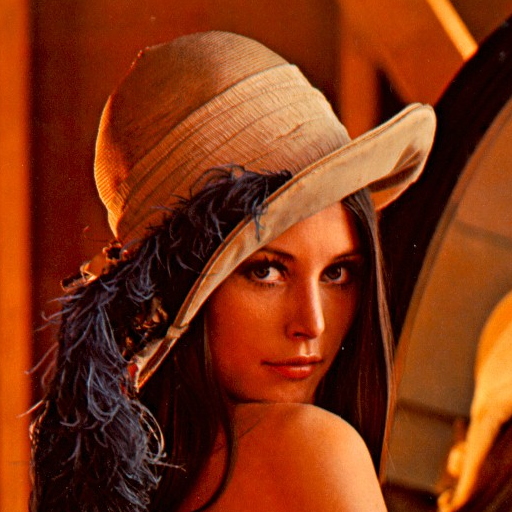
\includegraphics[width=0.9\textwidth]{lenna_1_original.png}
        \caption{Original Image}
        \label{fig:lena-original}
    \end{subfigure}
    \hfill
    \begin{subfigure}[b]{0.4\textwidth}
        \centering
        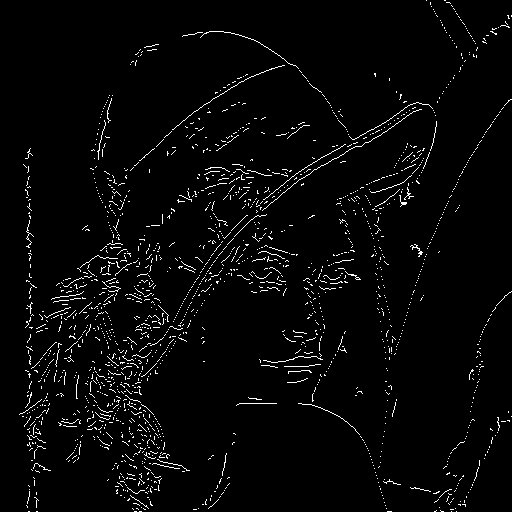
\includegraphics[width=0.9\textwidth]{lenna_8_canny_edge_detected.png}
        \caption{Edge Detected Image}
        \label{fig:lena-edge}
    \end{subfigure}
    \caption{Comparison of Original and Edge Detected Images using Canny Edge Detection Algorithm}
    \label{fig:lena-comparison}
\end{figure}

